% TorchDisorder — workflow and loss-balancing options
%
% Standalone TikZ document.  Build with:
%     pdflatex -output-directory=docs docs/workflow.tex
% (needs TikZ, amsmath, and the standalone class; all in TeX Live / MacTeX)
%
% The point of this figure is that the objective alone does not determine a
% structure.  Fitting a one-dimensional scattering curve is underdetermined, so
% the refinement is only meaningful together with the constraint terms and the
% validation gates.  Each box below names the config key that controls it, so a
% reader can trace any number in a run back to the switch that produced it.

\documentclass[border=12pt]{standalone}
\usepackage{tikz}
\usepackage{amsmath}
\usepackage{amssymb}
\usetikzlibrary{arrows.meta, positioning, fit, backgrounds, calc, shapes.geometric}

\definecolor{cData}{RGB}{ 37, 99,235}   % experimental input
\definecolor{cStruct}{RGB}{ 22,163, 74} % structural input
\definecolor{cLoss}{RGB}{217,119, 6}    % objective / loss
\definecolor{cBal}{RGB}{147, 51,234}    % balancing strategies
\definecolor{cGate}{RGB}{220, 38, 38}   % validation gates
\definecolor{cMuted}{RGB}{100,116,139}

\tikzset{
  box/.style   = {rounded corners=2pt, draw=#1, line width=0.9pt, fill=#1!5,
                  align=center, inner sep=6pt, font=\sffamily\small},
  eq/.style    = {align=left, font=\small, inner sep=4pt},
  key/.style   = {font=\ttfamily\scriptsize, text=cMuted},
  flow/.style  = {-{Stealth[length=5pt]}, line width=0.9pt, draw=cMuted},
  gate/.style  = {diamond, aspect=2, draw=cGate, line width=0.9pt, fill=cGate!5,
                  align=center, inner sep=2pt, font=\sffamily\scriptsize},
  hdr/.style   = {font=\sffamily\bfseries\large},
  note/.style  = {font=\itshape\scriptsize, text=cMuted, align=left},
}

\begin{document}
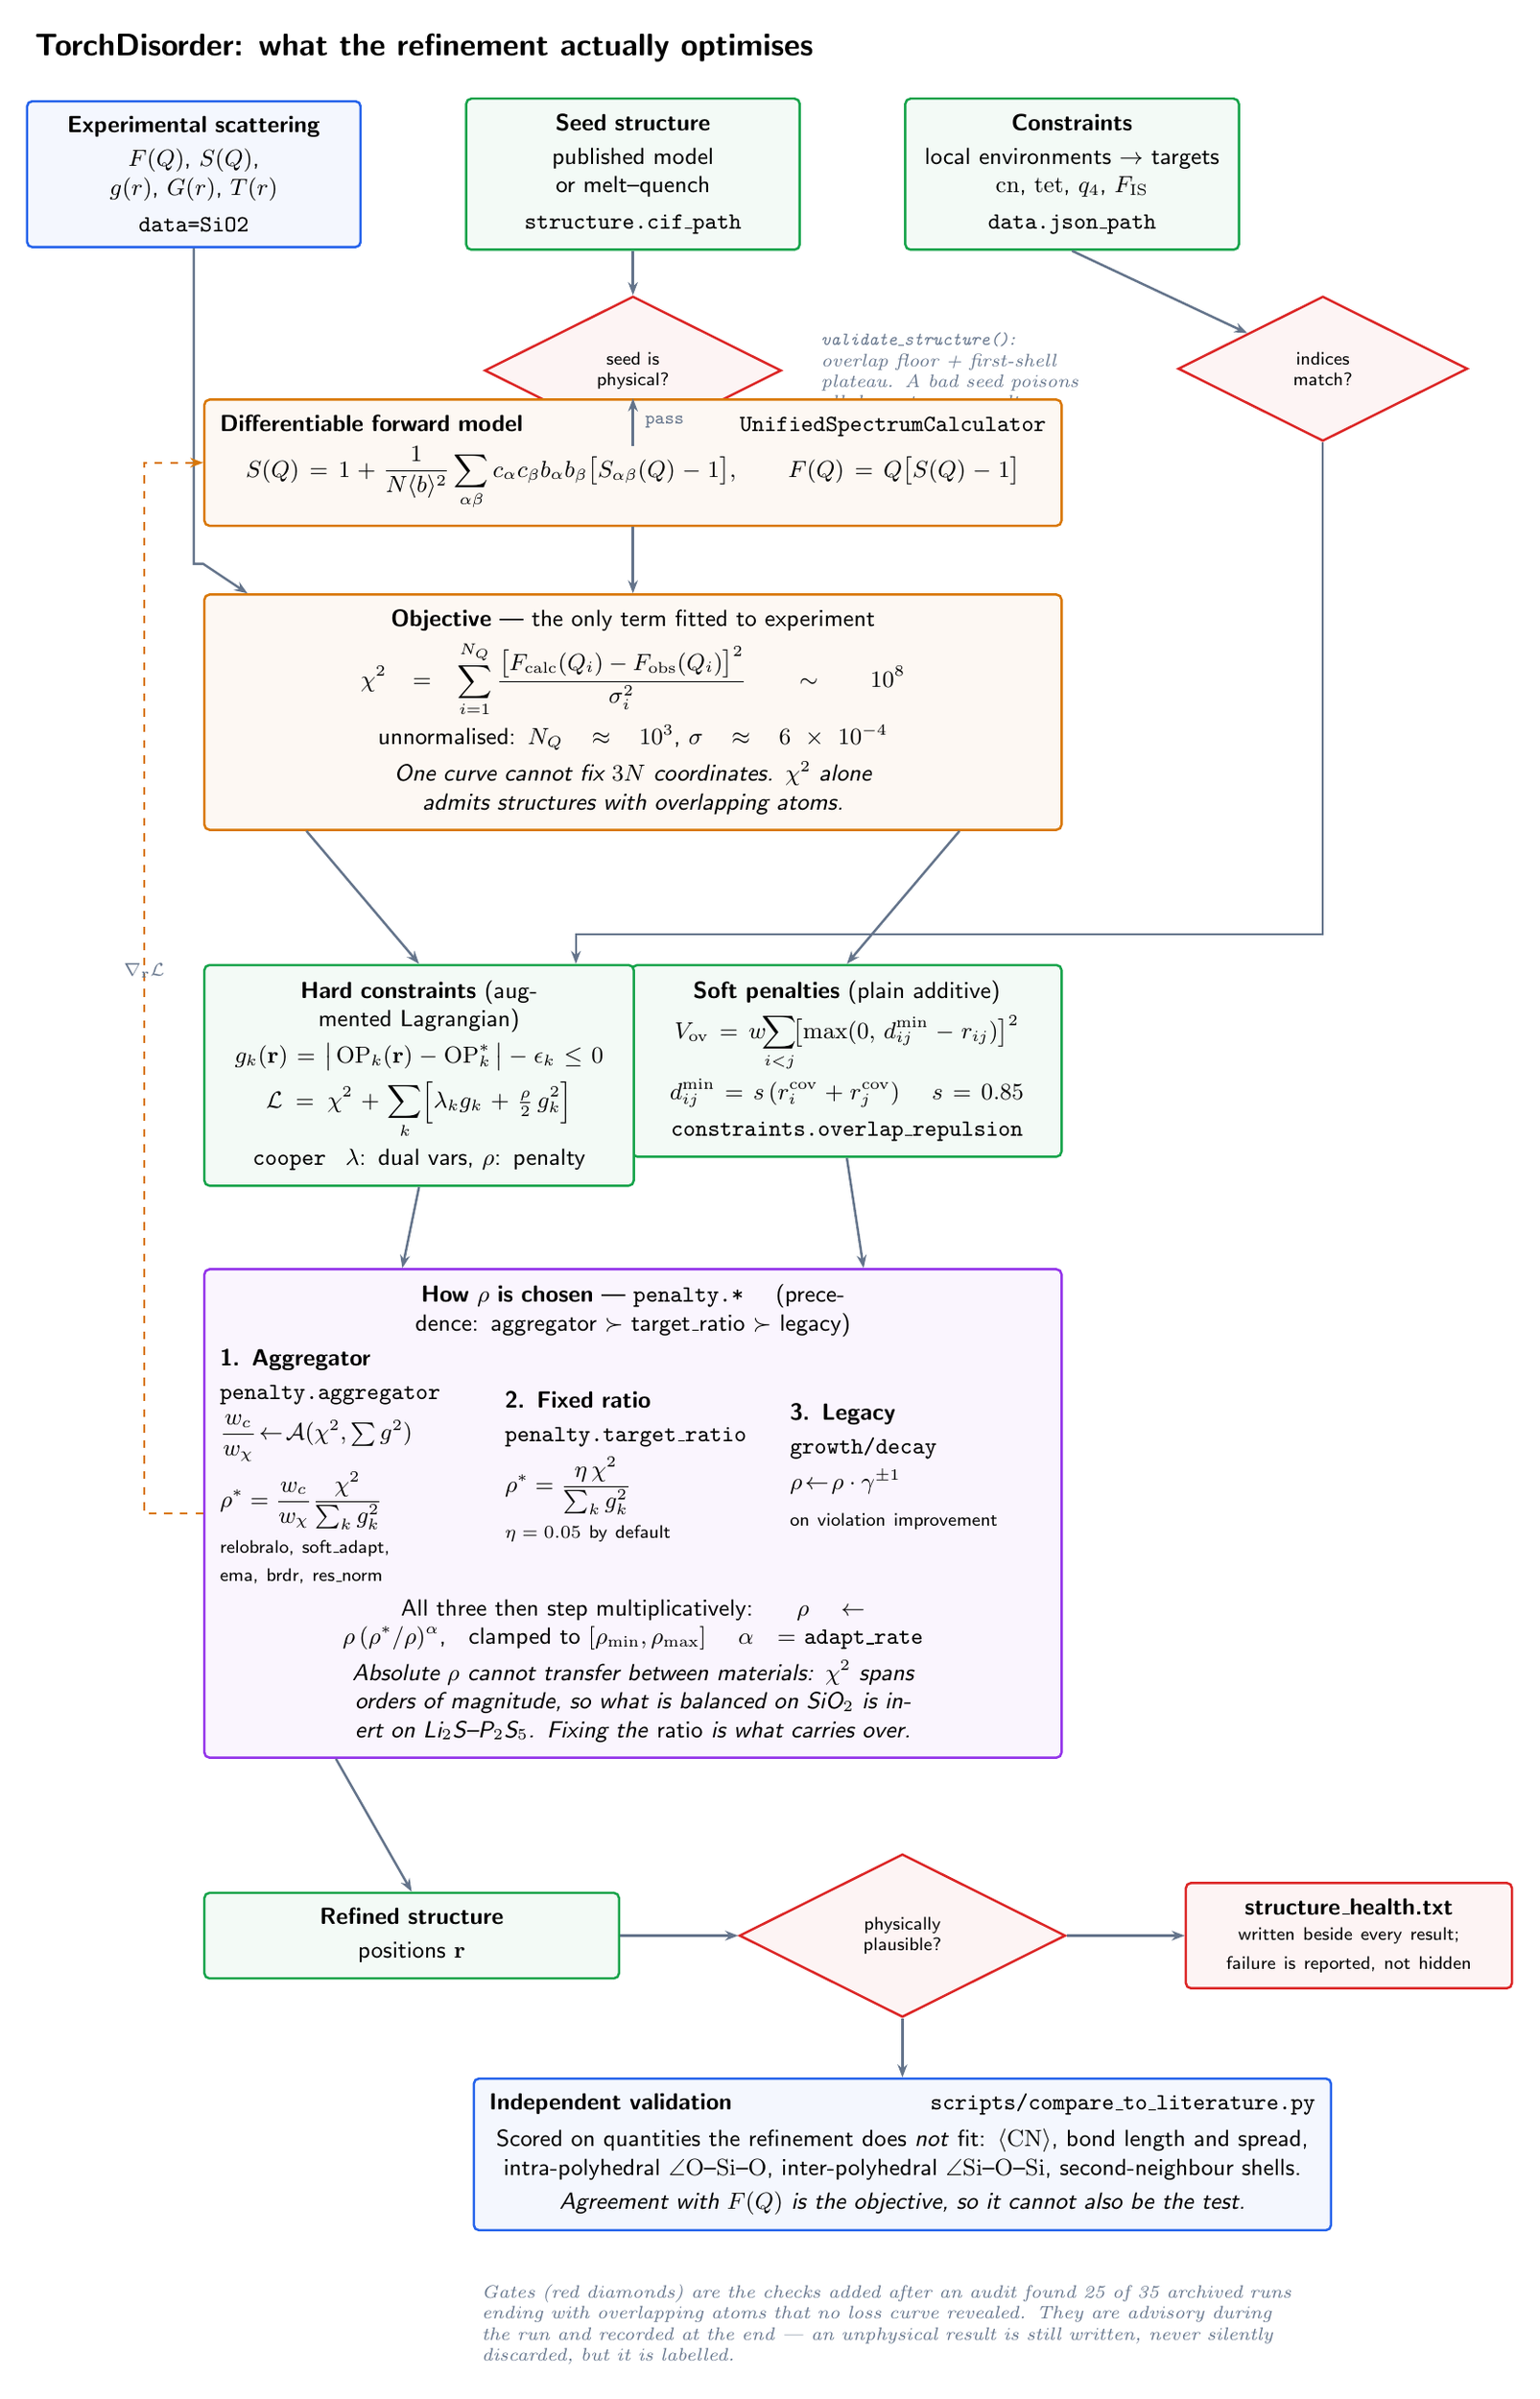
\begin{tikzpicture}[node distance=8mm]

% ─────────────────────────────────────────────────────────── inputs
\node[hdr] (title) {TorchDisorder: what the refinement actually optimises};

\node[box=cData, below=7mm of title.west, anchor=north west, text width=41mm]
  (data) {\textbf{Experimental scattering}\\[2pt]
          $F(Q)$, $S(Q)$, $g(r)$, $G(r)$, $T(r)$\\[3pt]
          {\ttfamily data=SiO2}};

\node[box=cStruct, right=14mm of data, text width=41mm]
  (seed) {\textbf{Seed structure}\\[2pt] published model or melt--quench\\[3pt]
          {\ttfamily structure.cif\_path}};

\node[box=cStruct, right=14mm of seed, text width=41mm]
  (cons) {\textbf{Constraints}\\[2pt] local environments $\to$ targets\\
          $\mathrm{cn}$, $\mathrm{tet}$, $q_4$, $F_{\mathrm{IS}}$\\[3pt]
          {\ttfamily data.json\_path}};

\node[gate, below=6mm of seed, text width=26mm] (gseed)
  {seed is\\physical?};
\node[note, right=4mm of gseed, text width=52mm, anchor=west] {%
  \texttt{validate\_structure()}:\\ overlap floor + first-shell\\ plateau.
  A bad seed poisons\\ all downstream results.};

\node[gate, below=6mm of cons, xshift=34mm, text width=26mm] (gidx)
  {indices\\match?};

% ─────────────────────────────────────────────────────────── forward model
\node[box=cLoss, below=20mm of seed, text width=112mm] (model)
  {\textbf{Differentiable forward model} \hfill {\ttfamily UnifiedSpectrumCalculator}\\[3pt]
   $\displaystyle
     S(Q)=1+\frac{1}{N\langle b\rangle^{2}}\sum_{\alpha\beta} c_\alpha c_\beta
     b_\alpha b_\beta \bigl[S_{\alpha\beta}(Q)-1\bigr],
     \qquad F(Q)=Q\bigl[S(Q)-1\bigr]$};

% ─────────────────────────────────────────────────────────── objective
\node[box=cLoss, below=9mm of model, text width=112mm] (chi)
  {\textbf{Objective} --- the only term fitted to experiment\\[3pt]
   $\displaystyle \chi^{2}=\sum_{i=1}^{N_Q}
      \frac{\bigl[F_{\mathrm{calc}}(Q_i)-F_{\mathrm{obs}}(Q_i)\bigr]^{2}}{\sigma_i^{2}}
      \;\sim\;10^{8}$\\[2pt]
   {\small unnormalised: $N_Q\approx10^{3}$, $\sigma\approx6\times10^{-4}$}\\[3pt]
   {\itshape One curve cannot fix $3N$ coordinates. $\chi^2$ alone admits
    structures with overlapping atoms.}};

% ─────────────────────────────────────────────────────────── constraint terms
\node[box=cStruct, below=9mm of chi, text width=54mm, anchor=north east]
  at ($(chi.south east)+(0,-9mm)$) (soft)
  {\textbf{Soft penalties} (plain additive)\\[3pt]
   $\displaystyle V_{\mathrm{ov}}=w\!\!\sum_{i<j}\!
     \bigl[\max(0,\,d^{\min}_{ij}-r_{ij})\bigr]^{2}$\\[2pt]
   $d^{\min}_{ij}=s\,(r^{\mathrm{cov}}_i+r^{\mathrm{cov}}_j)$ \quad {\small$s=0.85$}\\[3pt]
   {\ttfamily constraints.overlap\_repulsion}};

\node[box=cStruct, below=9mm of chi, text width=54mm, anchor=north west]
  at ($(chi.south west)+(0,-9mm)$) (hard)
  {\textbf{Hard constraints} (augmented Lagrangian)\\[3pt]
   $\displaystyle g_k(\mathbf{r})=\bigl|\,\mathrm{OP}_k(\mathbf{r})-\mathrm{OP}_k^{\ast}\,\bigr|-\epsilon_k \le 0$\\[3pt]
   $\displaystyle \mathcal{L}=\chi^{2}+\sum_k\Bigl[\lambda_k g_k
      +\tfrac{\rho}{2}\,g_k^{2}\Bigr]$\\[3pt]
   {\ttfamily cooper} $\;\lambda$: dual vars, $\rho$: penalty};

% ─────────────────────────────────────────────────────────── balancing
\node[box=cBal, below=11mm of hard.south west, anchor=north west, text width=112mm] (bal)
  {\textbf{How $\rho$ is chosen} --- {\ttfamily penalty.*} \quad
   {\small(precedence: aggregator $\succ$ target\_ratio $\succ$ legacy)}\\[4pt]
   \begin{minipage}{0.31\linewidth}
     \textbf{1. Aggregator}\\[2pt]
     {\ttfamily penalty.aggregator}\\[3pt]
     $\dfrac{w_c}{w_\chi}\!\leftarrow\!\mathcal{A}(\chi^2,\textstyle\sum g^2)$\\[3pt]
     $\rho^{\ast}=\dfrac{w_c}{w_\chi}\dfrac{\chi^{2}}{\sum_k g_k^{2}}$\\[3pt]
     {\scriptsize relobralo, soft\_adapt,\\ ema, brdr, res\_norm}
   \end{minipage}\hfill
   \begin{minipage}{0.31\linewidth}
     \textbf{2. Fixed ratio}\\[2pt]
     {\ttfamily penalty.target\_ratio}\\[3pt]
     $\rho^{\ast}=\dfrac{\eta\,\chi^{2}}{\sum_k g_k^{2}}$\\[3pt]
     {\scriptsize $\eta=0.05$ by default}
   \end{minipage}\hfill
   \begin{minipage}{0.31\linewidth}
     \textbf{3. Legacy}\\[2pt]
     {\ttfamily growth/decay}\\[3pt]
     $\rho\!\leftarrow\!\rho\cdot\gamma^{\pm1}$\\[3pt]
     {\scriptsize on violation improvement}
   \end{minipage}\\[5pt]
   All three then step multiplicatively:
   $\;\rho \leftarrow \rho\,(\rho^{\ast}/\rho)^{\alpha}$, \; clamped to
   $[\rho_{\min},\rho_{\max}]$ \quad {\small$\alpha=$ {\ttfamily adapt\_rate}}\\[3pt]
   {\itshape Absolute $\rho$ cannot transfer between materials: $\chi^2$ spans orders
    of magnitude, so what is balanced on SiO$_2$ is inert on Li$_2$S--P$_2$S$_5$.
    Fixing the \emph{ratio} is what carries over.}};

% ─────────────────────────────────────────────────────────── output + gate
\node[box=cStruct, below=9mm of bal, text width=52mm, anchor=north west]
  at ($(bal.south west)+(0,-9mm)$) (out)
  {\textbf{Refined structure}\\[2pt] positions $\mathbf{r}$};

\node[gate, right=16mm of out, text width=30mm] (gout) {physically\\plausible?};

\node[box=cGate, right=16mm of gout, text width=40mm] (report)
  {\textbf{structure\_health.txt}\\[2pt]
   {\scriptsize written beside every result;\\ failure is reported, not hidden}};

% ─────────────────────────────────────────────────────────── independent check
\node[box=cData, below=8mm of gout, text width=112mm] (lit)
  {\textbf{Independent validation} \hfill {\ttfamily scripts/compare\_to\_literature.py}\\[3pt]
   Scored on quantities the refinement does \emph{not} fit:
   $\langle \mathrm{CN}\rangle$, bond length and spread,
   intra-polyhedral $\angle\mathrm{O}\text{--}\mathrm{Si}\text{--}\mathrm{O}$,
   inter-polyhedral $\angle\mathrm{Si}\text{--}\mathrm{O}\text{--}\mathrm{Si}$,
   second-neighbour shells.\\[2pt]
   {\itshape Agreement with $F(Q)$ is the objective, so it cannot also be the test.}};

% ─────────────────────────────────────────────────────────── edges
\draw[flow] (seed) -- (gseed);
\draw[flow] (gseed) -- node[key,right=1pt]{pass} (model);
\draw[flow] (data.south) |- ($(chi.north west)+(0,4mm)$) -- ($(chi.north west)+(6mm,0)$);
\draw[flow] (cons.south) -- (gidx);
\draw[flow] (gidx.south) |- ($(hard.north east)+(-8mm,4mm)$) -- ($(hard.north east)+(-8mm,0)$);
\draw[flow] (model) -- (chi);
\draw[flow] ($(chi.south west)+(14mm,0)$) -- (hard.north);
\draw[flow] ($(chi.south east)+(-14mm,0)$) -- (soft.north);
\draw[flow] (hard.south) -- ($(bal.north west)+(27mm,0)$);
\draw[flow] (soft.south) -- ($(bal.north east)+(-27mm,0)$);
\draw[flow] (bal.south west) ++(18mm,0) -- (out.north);
\draw[flow] (out) -- (gout);
\draw[flow] (gout) -- (report);
\draw[flow] (gout.south) -- ++(0,-4mm) -| (lit.north);

% feedback loop: gradient step
\draw[flow, dashed, draw=cLoss]
  ($(bal.west)+(0,0)$) -- ++(-8mm,0) |- node[key, above, pos=0.25]{$\nabla_{\mathbf r}\mathcal{L}$}
  ($(model.west)+(-8mm,0)$) -- (model.west);

% ─────────────────────────────────────────────────────────── legend
\node[note, below=6mm of lit.south west, anchor=north west, text width=112mm] {%
  Gates (red diamonds) are the checks added after an audit found 25 of 35 archived
  runs ending with overlapping atoms that no loss curve revealed. They are
  advisory during the run and recorded at the end --- an unphysical result is
  still written, never silently discarded, but it is labelled.};

\end{tikzpicture}
\end{document}
